\documentclass[runningheads]{llncs}

\usepackage[T1]{fontenc}
\usepackage{cite}
\usepackage{graphicx}
\usepackage{graphicx} % Required for inserting images
\usepackage{hyperref}
\usepackage{float}
\usepackage{xcolor}
\usepackage{amsmath} % begin{aligned}
\usepackage{amsfonts} % \mathbb{}
\usepackage{todonotes} % \todo and \todo[inline]
\usepackage{paralist}
\usepackage{enumitem}

% Enumerator for Objectives
\newlist{objectives}{enumerate}{2}
\setlist[objectives,1]{label=O\arabic*.,ref=O\arabic*}
\setlist[objectives,2]{label=(\alph*),ref=\thequestionsi(\alph*)}

\newcommand{\xor}{\oplus}
\newcommand{\toref}[1]{\todo[color=yellow]{#1}}
\newcommand{\tothink}[1]{\todo[color=pink]{#1}}


\begin{document}
	
	\title{Generating trusted sphinx packets}
	
	\author{Anonymous}
	\authorrunning{Anonymous}
	\institute{}
	
	\maketitle 
	
	\begin{abstract}
		We propose a decentralized scheme that prevent mixnets users from sending traffic that does not match the service provider of an anonymous credential. Our scheme is of direct use in the Nym network where users construct an anonymous credential given they receive a certificate of them paying for that service provider. Our scheme prevent users from cheating by using a credential for a free service and send traffic for a paid service. Our solution works even if the majority of the third parties collude. Finally we evaluate the performance of our solution.
		\keywords{mixnet \and sphinx \and malicious users}
	\end{abstract}


\section{Introduction}

Mix network, or mixnet, is an overlay network of servers (called mix nodes) that prevent an adversary from correlating senders with receivers~\cite{chaum-mix,cypherpunk-remailer,piotrowska2017loopix,nym-network-whitepaper,danezis2003mixminion, van2015vuvuzela,mixmaster-spec,chaum2016cmix}. They achieve this by adding delays to messages inside the different mixnodes in order to mitigate timing analysis attacks. Additionally, unlike Tor~\cite{onion-routing96} where all packets sent by a user follow the same path for the entire session (called circuit-based), in mixnets routing is typically packet-based (meaning that each packet follows a different path). These two techniques ensure that mixnets are resilient against a strong adversary who observes the entire input and outputs of the network typically called a Global Passive Adversary (GPA).
During the last few decades several systems have been proposed in the literature and few of them have been implemented. Open research problems such as parametrization, authentication and fake dummies have halted the usage on a large scale. Recently, Nym Technologies a mixnet-based company is being commercialized and proposing a mixnet network for services to be integrated with their network for a fee. Their network is based on Loopix~\cite{piotrowska2017loopix}. Users of these services are then allowed to use the nym mixnet by using Nym credentials (based on the Coconut credential~\cite{coconut}) that they can construct after getting a certificate of paying for a specific service to use the Nym network. However, nothing prevents users from cheating who might exploit a valid Nym credential for another service they did not pay for. This is a particular difficult problem in anonymous communication networks where the mixnodes do not know the traffic type or the final service a user is communicating with by doing layered encryption where the final IP address is only know by the last node in the path using a packer format such as Sphinx~\cite{sphinx}. 

In this paper we present a scheme that creates the Sphinx header in a
decentralized way based on trusted third parties while ensuring that these
parties learn nothing about the destination or the path. Our work makes the
following contributions:
%
\begin{itemize}
%
  \item{\ldots}
%
  \item{\ldots}
%
  \item{We assess the impact on availability and economic viability
adversaries can have in Sphinx and our solution and conclude that\ldots}
%
\end{itemize}
%
\todo{Something on prototype and availability of artifacts!}

We highlight related work and motivation in Section~\ref{sec:related}, then we specify and justify our system model in Section~\ref{sec:sys_model}, where we also describe the considered threat model. We then present our scheme that decentralize the creation of the Sphinx headers in Section~\ref{sec:scheme} and the evaluation of our proposed solution in Section~\ref{sec:eval}. Finally we conclude and discuss future work in Section~\ref{sec:conclusion}

\section{Motivation and Related Work}~\label{sec:related}
Since Chaum’s seminal work on untraceable email in 1981~\cite{chaum-mix}, there has been a great amount of research re
lated to mixnets' design~\cite{piotrowska2017loopix, van2015vuvuzela, kwon2020xrd, lazar2018karaoke, cottrell1995mixmaster, alexopoulos2017MCMIX, chaum2016cmix, chaum-mix, danezis2003mixminion}. However most systems that have been deployed and used come with their own system on top of the network meaning that only one type of traffic type is allowed. As beautifully stated by Dingledine et al. in~\cite{dingledine2006anonymity}, "Anonymity Loves Company" meaning that the more messages there are in the network the more privacy the network provide. This is also shared by Ben Guirat et al. in~\cite{benguirat2023blending} where the authors show that bledning different traffic types on top of a mixnet provide better anonymity, meaning let's imagine an instant messaging system where users do not tolerate latency of more than few seconds and an email app where users tolerate latency of up to 1 minute. The authors show that blending these two types of traffic do actually increase the privacy for both of traffic. This only applicable in networks such as Tor or the Nym network that they offer the network for different applications to be integrated on top of the network rather than dictating which application to use the mixnet.
However, certain open research problems remain open. For example how can we ensure that certain traffic are not allowed (for whatever reason and we will specify the exact reason for our work) without compromising ?
Tor solves the problem with having exit policy that simply drop traffic at the last node. However Tor routing is circuit-based meaning that all traffic from a specefic user session follow one path and hence packets are encrypted using symetric cryptographhy which is cheap, so even if traffic is dropped that is not a problem.

However unlike tor, mixnets can be expensive due to the routing type which is packet based , meaning that every packet takes a different path and hence layered encrypted using public key cryptography. This means that if packets are dropped at the lost nodes when not allowed, this waste a huge amount of cryptographic power. Additionally unlike tor where relay are volunteer based, nodes in mixnets such as Nym are economically incentivized based on the bandwidth they routed so if packets are dropped at the end this is not great.
\todo{Iness: add a simple graph here of a mixnet}

\section{System and Threat Model}~\label{sec:sys_model}
\subsection{System Model}



For example let's say Signal is integrated with Nym, and Signal users who want their traffic to be anonymous instead of sending traffic directly to the Signal server, traffic will be first routed through the mixnet such that an adversary who observes the signal server and/or the device of the user can not correlate the sender with signal server and evetually the final recepient. Signal (service provider) can add an option for user who want to pay and issue a certified attribute to those users. Users then encode this attributes into a credential and sends it to validators. If the proof is valid, validators return partial signatures. Once the user collects a threshold number of these signatures, they aggregate them to form a valid credential and re-randomize it to ensure unlinkability from previous interactions. The user can then present this credential to a verifier to prove their right to access a service to show that the credential meets all necessary payment and authentication conditions. To prevent double-spending, the verifier checks that the credential has not already been used by consulting the blockchain and then commits the credential's serial number to the blockchain upon acceptance.
For example, a user can obtain an certification from the Signal service provider, construct a valid credential and then use it to route traffic to another service provider they didn't pay for or simply not allowed (an illegal website).
Such misuse would be detected only at the final node of the mixnet preventing the user from accessing another application. 
However, prior mixnodes would have already wasted computational resources processing an invalid packet. 
This vulnerability enables Denial of Service (DoS) attack by exhausting mixnodes computational power with illegitimate packets.

Additionally, each encryption layer includes an integrity tag, which prevents tampering and improves the network’s resistance against malicious mixnodes and active adversaries.
This means that each packet follows a different path rather than using the same intermediate nodes during the whole communication.
 
To further prevent correlation, mixnet relies on fixed-size packet format such as Sphinx packet (section \ref{sec:sphinx}), making it difficult for external observers to link incoming and outgoing messages at any given node.
In summary, mixnets provide stronger privacy guarantees than onion routing at the cost of increased latency.


\subsection{Threat Model}
\section{Sphinx}\label{sec:sphinx}

Sphinx packets consist of a header and an encrypted payload. 
The header itself contains a \textit{cryptographic element $\alpha$} (e.g. $g^x$ or an elliptic curve point), \textit{encrypted routing information $\beta$}, and an \textit{integrity tag $\gamma$}, as illustrated in Figure \ref{fig:sphinx_structure}.

\begin{figure}[h]
    \centering
    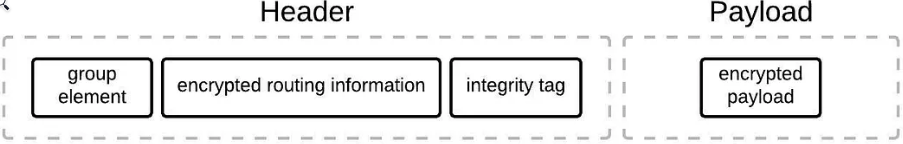
\includegraphics[width=0.9\linewidth]{Images/sphinx_structure.png}
    \caption{Structure of sphinx packet. \href{https://blog.nymtech.net/sphinx-tl-dr-the-data-packet-that-can-anonymize-bitcoin-and-the-internet-18d152c6e4dc}{[source]}}
    \label{fig:sphinx_structure}
\end{figure}

The \textit{encrypted routing information ($\beta$)} is constructed in layers, applied in reverse order along the path.
First, the final destination is encrypted, and an integrity tag ($\gamma_i$) is computed. 
The IP address of the last mixnode ($n_i$) is then prepended.
As shown by Figure \ref{fig:sphinx_header}, this process repeats iteratively: each new header is encrypted, an integrity tag ($\gamma_{i-1}$) is computed, and the IP address of the preceding mixnode ($n_{i-1}$) is prepended.
This layered encryption ensures that each mixnode can only decrypt its own layer, revealing the next forwarding address while preserving end-to-end confidentiality and protecting against tampering.

\begin{figure}[h]
    \centering
    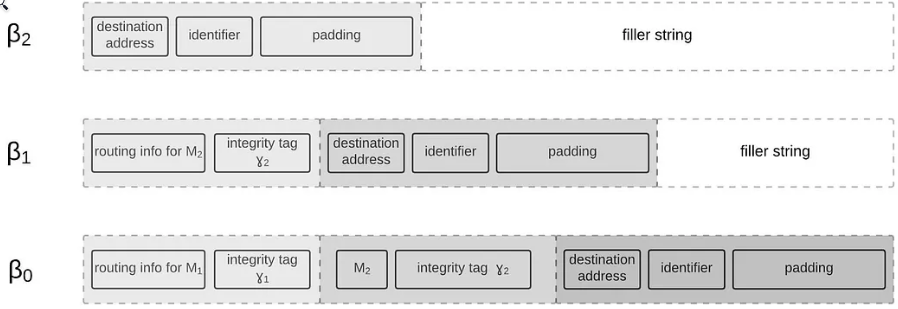
\includegraphics[width=\linewidth]{Images/sphinx_header.png}
    \caption{Sphinx encrypted routing information encapsulation. \href{https://blog.nymtech.net/sphinx-tl-dr-the-data-packet-that-can-anonymize-bitcoin-and-the-internet-18d152c6e4dc}{[source]}}
    \label{fig:sphinx_header}
\end{figure}

To encrypt the routing information, the nym client\todo{previously "user" but JT prefers "nym client"} first chooses a nonce $x$ and compute $\alpha = g^x$ as the \textit{cryptographic element} of the header.
Since each mixnode $i$ has a private key $x_i$ and a public key $y_i = g^{x_i}$, the user can create a shared secret $s_i$ with mixnode $i$ as followed: $s_i = y_i^x = (g^{x_i})^x$. 
Then the mixnode $i$ receiving the packet will get $\alpha$ allowing him to compute the shared secret as followed: $s_i = \alpha^{x_i} = (g^x)^{x_i}$.

Instead of sending a unique \textit{cryptographic element $\alpha$} at each node in the path, the sphinx format uses a single \textit{cryptographic element $\alpha$}, which is progressively modified at each node. 
Each mixnode updates the cryptographic element using its shared secret as follows:  
$$\alpha_{i+1} = \alpha_i^{\text{hash}(\alpha_i, s_i)}$$
Thus, the user iteratively computes the shared secrets in the path's order as: 
$$
\begin{aligned}
    \alpha_0 &= g^{x}, & s_0 &= y_{n_0}^{x}, & b_0 &= \text{hash}(\alpha_0, s_0) \\
    \alpha_1 &= g^{x b_0}, & s_1 &= y_{n_1}^{x b_0}, & b_1 &= \text{hash}(\alpha_1, s_1) \\
    &\vdots & &\vdots & &\vdots \\
    \alpha_i &= g^{x b_0 \cdots b_{i-1}}, & s_i &= y_{n_i}^{x b_0 \cdots b_{i-1}}, & b_i &= \text{hash}(\alpha_i, s_i)
\end{aligned}
$$
This formulation ensures that each mixnode can independently derive the necessary cryptographic elements without requiring the full path’s information, preserving privacy and unlinkability.  
\newline

The \textit{encrypted routing information ($\beta$)} is computed, as illustrated in Figure\todo{$\sim$\textbackslash ref\{\}} \ref{fig:sphinx_header}, by processing the path in reverse order. 
This involves XORing the routing information ($\beta_{i-1}$) from the previous layer (with the node's address and integrity tag) with a value derived from the shared secret $s_i$. 
Then prepending this new encrypted routing information ($\beta_i$) with an integrity tag ($\gamma_i$) and the previous mixnode address (remember we build it in reverse order).
We repeat the same process for each layer (i.e. each mixnode in the path).

\begin{figure}[H]
    \centering
    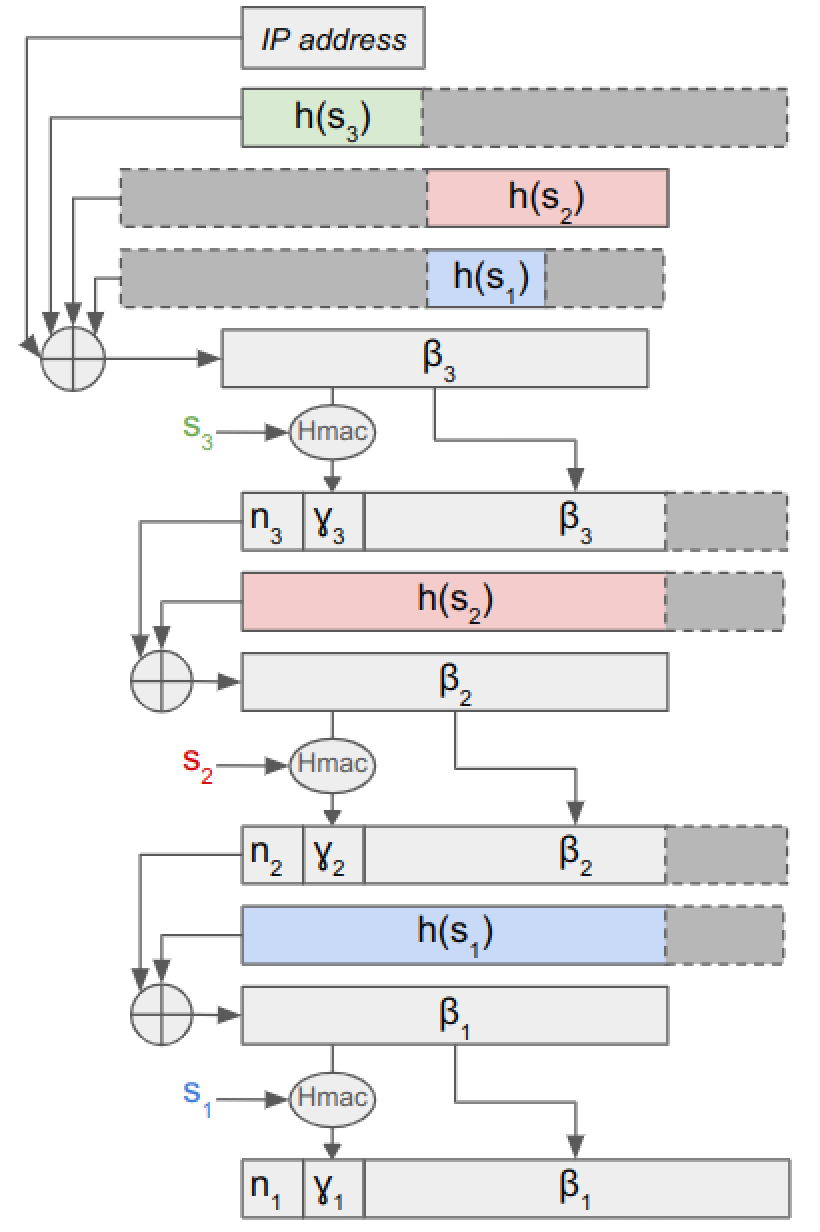
\includegraphics[width=0.5\linewidth]{Images/header_cipher.png}
    \caption{Construction of the Sphinx header (modified from \cite{sphinx}) [TO FIX: $h(s_1)$ at first XOR]}
    \label{fig:header_cipher}
\end{figure}
\todo[inline]{JT: Explain what the modifications are}
\todo[inline]{JT: Might help to put some (1) (2) (3) labels into the figure and refer to these labels in the text.}

% first round
The first round of XOR operations differs from the others because it requires combining parts of all shared secrets. 
Specifically, the destination address is XORed with the last node’s shared secret, truncated to match the address size.
Next, the result is concatenated with the XORed values of the ending parts of the shared secrets from the other nodes in the path. 
This ensures that when the entire header is XORed with the full shared secret, these appended values cancel out, allowing the header to be processed in reverse order by the mixnodes.
This design choice guarantees fixed-size headers, enabling fixed-size packets which is a crucial property in mixnets for maintaining unlinkability.

\todo[inline]{JT: Now maybe follow up with an example of the attack from the introduction?
We should also compare computational overheads from attack vs. the new protocol design.}



\section{Multi-Party Computation (MPC)}

The first approach to ensuring trust in the Sphinx header is to prevent user manipulation by decentralizing the header construction to Trusted Third Parties (TTP) through the use of Multi-Party Computaftion (MPC).

We consider TTPs as \textit{honest-but-curious}.\tothink{What if malicous TTP...}
This means that they follow the protocol correctly but may attempt to infer additional information from the data they process.
Our design aims to ensure that TTPs must not be able to infer any information about the shared secrets $s_i$ nor the mixnodes involved in the path, even when TTP are colliding (assuming that at least one TTP remains honest).
\todo{JT: In the Nym ecosystem, who are the TTPs, who operates them, what exactly are they trusted for?}
\newline


% Overall path selection:
% 1) Users choose the path
% 2) TTP randomly choose the path (without knowing it)

% Overall schema 
% 1̶)̶ ̶O̶n̶e̶ ̶T̶T̶P̶ ̶p̶e̶r̶ ̶l̶a̶y̶e̶r̶
% 2) TTP do a layer, then aggregate, then next layer  => What if user send h(s_i) ?! (TODO)
% 3) TTP do the whole computation then aggregate
To decentralize the construction of the Sphinx header, we first examined how to partition and distribute the computation. 
Three approaches were considered.

The first and most naive approach involves that each TTP computes a different layer of the header. 
This approach reveals two consecutive nodes in the path and one of the corresponding shared secrets ($s_i$) at each TTP, leading to serious security concerns in the case of collusion.

In a second approach, the user sends to each TTP a piece of the destination address.
Each TTP computes the same layer on its partial destination.
The resulting partial headers of this layer are aggregated to compute the integrity tag. 
This process is repeated layer by layer. 
However, computing the integrity tag at the end of each layer requires knowledge of the shared secret $s_i$. 
\tothink{User could send $h(s_i)$ to TPP such that it could computes the integrity check without getting useful information...}
If a TTP does it, it reintroduces the same problem as the first approach.
If the user does it, he could potentially cheat.

The third and retained approach is similar to the second one.
Instead of partial computations at each layer, each TTP computes a full Sphinx header using only its assigned partial destination. 
These partial headers are then returned to the user, who aggregates them to produce the final Sphinx header.
Although this approach requires less interaction with the TTPs, it introduces additional constraints as discussed in section \toref{ref section}.
\todo{JT: I think we should only focus on the third approach.
There could be a section "Alternative Designs" where we discuss your other approaches.}

The overall decentralized scheme is illustrated in Figure \ref{fig:overall_schema}. 
The user begins by splitting the destination into several parts, such that their combination (e.g., via XOR) reconstructs the original address. 
Each part is sent to a different TTP, along with the required cryptographic material. 
The TTPs independently generate Sphinx headers using a modified version of the protocol. \toref{(see section ...)} 
These partial headers are then returned to the user, who aggregates them to form the final Sphinx header, ready for transmission through the mixnet.

\begin{figure}[H]
    \centering
    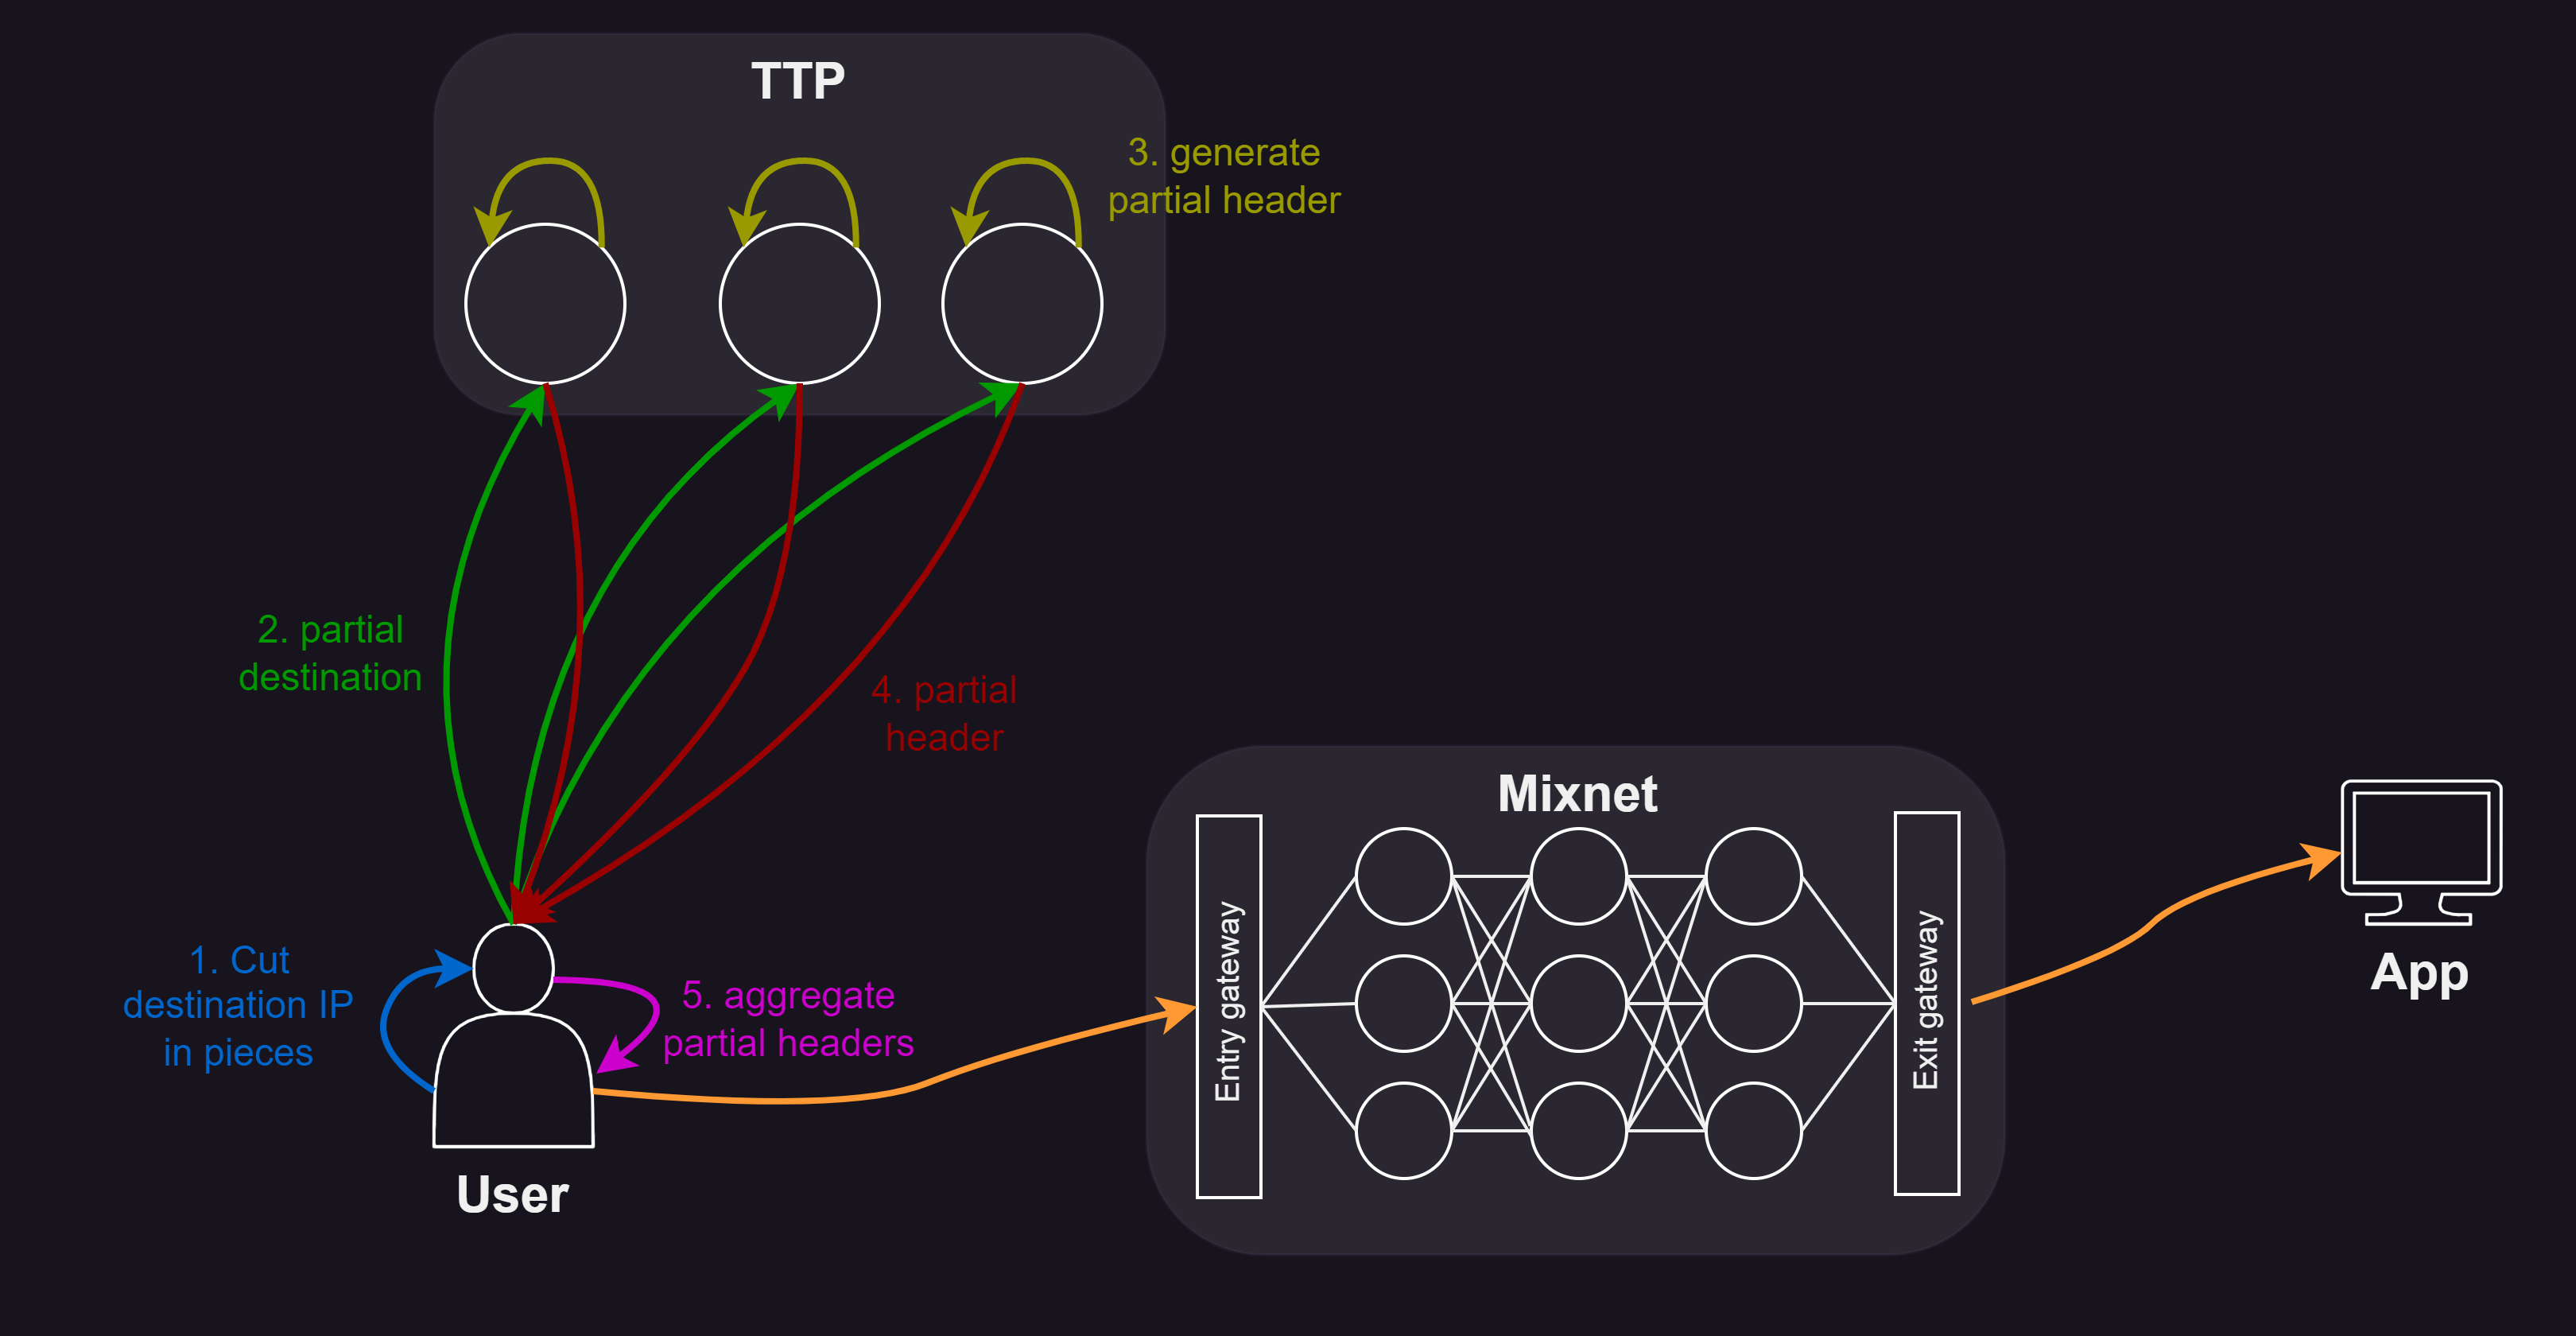
\includegraphics[width=0.5\linewidth]{Images/sphinx_ttp.png}
    \caption{Overview of the decentralized scheme\todo{Iness: Is there a reason why the arrows have different colors? If not than change to all black, Change "App" with "Service provider", Also I prefer a white background over black}}
    \label{fig:overall_schema}
\end{figure}

%%%%%%%%%%%%%%%
%One major challenge in decentralizing the original sphinx schema (Figure \ref{fig:header_cipher}) lies in the integrity tag, which is computed as the HMAC of the header $\beta_i$ using shared secret $s_i$. 
%To ensure security, no third party should have access to $s_i$, as collusion among third parties could lead to the recovery of all $s_i$, enabling them to decrypt the header and payload.
%To address this, third parties could compute a portion of the HMAC using a fragment of the shared secret $s_i$, and then combine these partial HMACs to produce the final HMAC. 
%This approach would require a hash function with homomorphic properties, which inherently weakens the collusion resistance and potentially compromises the second pre-image resistance of a secure hash.
%%%%%%%%%%%%%%%

\todo{I'd rather specify the requirements for the hash here.}
The main issue with the choosen approach is that we have to compute integrity tag on partial header such 
that combining those partial integrity tag gives the integrity tag of the final header.
However, even if breaking this homomorphic hash is feasible, if it remains computationally hard enough (e.g., requiring several hours), it could still be considered sufficiently secure for our purposes.
% TODO: VERIFY WHY NEED TO BE PER CHUNK
% What append if size secret bigger than chunk size (more random ?)


% ALPHA - 3 possibilities
% 1) Sending 1 alpha that is derived at each mixnode to generate a new alpha (efficient and clean but maybe not random enough)
    %  a) $\alpha_{i+1} = \alpha_i^{hash(\alpha_i, s_i)}$  -> article version
    %  b) $\alpha_{i+1} = G^{hash(\alpha_i, s_i)}$  --> Avoid "(x*b) % (mod-1)" in the exp -> less constraints
    %  c) $\alpha_{i+1} = \alpha_i^{2 s_i+1}$
    %  D) $\alpha_{i+1} = G^{\alpha_i (2 s_i+1)}$
% 2) Sending 1 alpha (unchanged) that is encrypted at each mixnode for the next one node (slower)
% 3) Sending 3 alpha (esay, robust but not size efficent) 

% BETA
% 1) compute by chunk
% 2) compute the whole ==> Possible ? If yes/no on which cases 

% GAMMA
% 0) User sends hash(s_i) if computed by layer
% 1) Using a different secret (s'_i) for integrity that is common to all TTP (for RSA) ==> i.e. different message, same secret
        % Pro: Easier
        % Con: Need an extra secret to send and key to handle
% 2̶)̶ ̶U̶s̶i̶n̶g̶ ̶p̶a̶r̶t̶i̶a̶l̶ ̶s̶_̶i̶ ̶o̶n̶ ̶p̶a̶r̶t̶i̶a̶l̶ ̶b̶e̶t̶a̶_̶i̶ ̶=̶=̶>̶ ̶i̶.̶e̶.̶ ̶d̶i̶f̶f̶e̶r̶e̶n̶t̶ ̶m̶e̶s̶s̶a̶g̶e̶,̶ ̶d̶i̶f̶f̶e̶r̶e̶n̶t̶ ̶s̶e̶c̶r̶e̶t̶
        %̶ ̶e̶.̶g̶.̶ ̶(̶s̶_̶i̶1̶ ̶*̶ ̶b̶'̶_̶i̶1̶)̶ ̶*̶ ̶(̶s̶_̶i̶2̶ ̶*̶ ̶b̶'̶_̶i̶2̶)̶ ̶*̶ ̶(̶.̶.̶.̶)̶ ̶=̶=̶>̶ ̶b̶'̶ ̶m̶u̶s̶t̶ ̶b̶e̶ ̶t̶h̶e̶ ̶f̶r̶e̶s̶h̶ ̶c̶o̶m̶p̶u̶t̶e̶d̶ ̶b̶ ̶(̶n̶o̶t̶ ̶t̶h̶e̶ ̶p̶r̶e̶v̶i̶o̶u̶s̶ ̶o̶n̶e̶)̶
        % /!\ LEAK INFORMATION (about s_i) /!\

% %\section{Zero-Knowledge Proof (ZKP)}

If we focus solely on the final encrypted routing information ($\beta$), we can simplify the diagram from Figure \ref{fig:header_cipher} to the representation in Figure \ref{fig:schema_final_header}.
\footnote{It is important to note that Figure \ref{fig:schema_final_header} shows the final representation of the encrypted routing information, not the computation, as the integrity tags ($\gamma$) still need to be computed.}
We observe that a small part of the header contains the destination address ($\delta$) XORed with part of each shared secret. 
In other words, a substring $\beta^*$ of the final header is equal to $\Delta \xor h(s_3) \xor h(s_2) \xor h(s_1)$.

\begin{figure}[H]
    \centering
    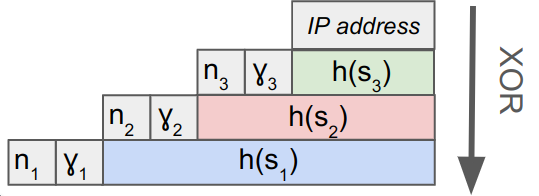
\includegraphics[width=0.5\linewidth]{Images/structure_final_header.png}
    \caption{Representation of the final encrypted routing information ($\beta$)}
    \label{fig:schema_final_header}
\end{figure}

Therefore, to user could prove that the destination address used in the original header is indeed the one he is authorized by its credentials (i.e. to one linked to its credential) without revealing anything about neither the destination, neither the routing path. 
In other words, proving that the $\Delta$ linked to the credential is the one used in $\beta^*$ = $\Delta \xor h(s_3) \xor h(s_2) \xor h(s_1)$.
To recall, with the current Sphinx mixnet architecture, a user can specify any destination address $\Delta$, and the packet will still traverse the entire mixnet before the fraud is detected at the exit gateway.

\paragraph{Idea} Proving that the address $\Delta$ from the credentials is indeed the one used in the header (i.e. $\beta^* = \Delta \xor h(s_3) \xor h(s_2) \xor h(s_1)$).

\paragraph{Limitations} Zero-Knowledge proofs are efficient with addition and multiplication operators, but not with the XOR (bitwise) operator, as XOR requires a separate proof for each bit instead of a single proof for the entire operation.

\paragraph{Solutions} To improve the efficiency of the ZKP proof, we could replace the XOR in the original schema (Figure \ref{fig:header_cipher}) with modular addition, measuring performance improvement, and ensuring it does not compromise security.

\paragraph{Discussion} If a user want to exhaust mixnode computation, he can provide the right $\Delta$ with a wrong $h(s_3)$. 
This strategy would exhaust the computational resources of the first two mixnodes before being detected at the third one, just before the exit gateway (one hop earlier that previously).
Thus we should look at a way to proof that $h(s_3)$ is correct as well... % ECC schema, Homomorphic Hash, in the construction of mixnode key that could be verified ???
Otherwise, we can think of it differently. 
Is it really a problem if user exhaust mixnodes computation ? 
It depends, in case of light network traffic is not a big deal since it follows the role of 'dummy' packet, improving the anonymity.

\section{Evaluation}\label{sec:eval}


\subsection{Discussion}

\todo[inline]{Come back to \ref{sec:sp-objectives} objectives and explain
why they hold.}



\section{Conclusion}\label{sec:conclusion}


\bibliographystyle{splncs04}
\bibliography{bib}

\end{document}
